\documentclass[conference]{IEEEtran}
\usepackage{cite}
\usepackage{amsmath,amssymb}
\usepackage{graphicx}
\usepackage{textcomp}
\usepackage{xcolor}
\usepackage{booktabs}
\usepackage{array}
\usepackage{tikz}
\usetikzlibrary{positioning,arrows.meta}
\usepackage{pgfplots}
\pgfplotsset{compat=1.18}
\usepackage{hyperref}

\definecolor{forest}{HTML}{2A78D6}
\definecolor{neutral}{HTML}{8A8880}
\definecolor{seriesb}{HTML}{EB6834}

\begin{document}

\title{Supervised Classification of Sensor Faults and Weather Extremes in Automatic Weather Station Networks}

\author{\IEEEauthorblockN{Jeetaksh Luhaniwal}
\IEEEauthorblockA{B.Tech CSE (AI/ML)\\
Lovely Professional University\\
Phagwara, Punjab, India\\
manojjeetakshluhaniwal25@gmail.com}}

\maketitle

\begin{abstract}
A faulty sensor in an automatic weather station quietly corrupts every forecast and alert built on
it, yet a genuine heat wave or storm can look just as unusual as a broken instrument. This paper
treats the problem as supervised classification. One year of hourly ERA5 reanalysis for eight
Indian cities (280{,}320 readings over four sensors) is augmented with six labelled sensor-fault
types and four seasonal, physically coherent extreme-weather types. Sixteen features describe each
reading, including how the other sensors of the same station are moving, and a Random Forest assigns
one of eleven classes. Evaluated with station-grouped cross-validation, so that every reading is
predicted by a model that never saw its station, the classifier reaches 97.9\% accuracy, 83.4\%
balanced accuracy and a macro F1 of 0.877 on the normal/fault/extreme task, against 94.3\%, 44.2\%
and 0.485 for a fixed range check. Eleven-class accuracy is 97.3\%. We report the majority-class
baseline (93.0\%) alongside every accuracy figure and discuss the classes that remain hard.
\end{abstract}

\begin{IEEEkeywords}
supervised learning, random forest, sensor fault detection, weather stations, extreme events,
data quality.
\end{IEEEkeywords}

\section{Introduction}
Automatic weather stations feed numerical forecasts, agricultural advisories and disaster warnings.
When a sensor fails loudly, for example by reporting a temperature of 200\,\textdegree C, a fixed
range check catches it. Most failures are quieter: a sensor sticks at one value, drifts by a few
degrees over a week, or loses precision. These readings stay inside physical limits and pass
unnoticed.

The opposite error matters just as much. A heat wave pushes temperature far above its seasonal
level, and a naive quality check that flags every unusual reading would discard exactly the data
that disaster response needs. A useful system must therefore answer two questions for every
reading: \emph{is it unusual}, and \emph{is the instrument at fault or is the weather genuinely
extreme}.

We frame both questions as one supervised classification problem with eleven classes: normal, six
fault types and four extreme types. The contributions are:
\begin{itemize}
\item a labelled benchmark built by injecting realistic faults and seasonal extremes into one year
of real ERA5 weather for eight climatically diverse Indian stations;
\item sixteen interpretable features, including station-level features that capture whether several
sensors move together, which is the physical signature separating weather from faults;
\item a Random Forest classifier evaluated with station-grouped cross-validation, reported against
both a majority-class baseline and the operational range check.
\end{itemize}

\section{Related Work}
Sensor faults in environmental networks have been catalogued by Ni \emph{et al.}~\cite{ni2009} and
measured in real deployments by Sharma \emph{et al.}~\cite{sharma2010}, who identify short spikes,
constant (stuck) readings and noise as the most common types. Operational meteorology relies on
rule-based quality control such as range, step and persistence tests~\cite{wmo2004,durre2010}. These
rules are transparent but cannot tell a real extreme from a fault.

Unsupervised anomaly detection~\cite{chandola2009}, including Isolation Forest~\cite{liu2008},
avoids labels but only reports \emph{how} unusual a reading is, not \emph{why}. When labelled
examples are available, supervised tree ensembles are a strong default for tabular
data~\cite{grinsztajn2022}, and Random Forests~\cite{breiman2001} in particular offer robustness to
feature scaling and built-in importance estimates. Because real labelled failure logs are rarely
published, fault injection into clean data is the standard way to build benchmarks~\cite{sharma2010}.

\section{System Overview}
Fig.~\ref{fig:pipeline} shows the pipeline. Two Python scripts hold the whole method:
\texttt{generate\_data.py} builds the labelled dataset and \texttt{model.py} builds features, trains
and evaluates the classifier, and writes the files that a web dashboard displays.

\begin{figure}[t]
\centering
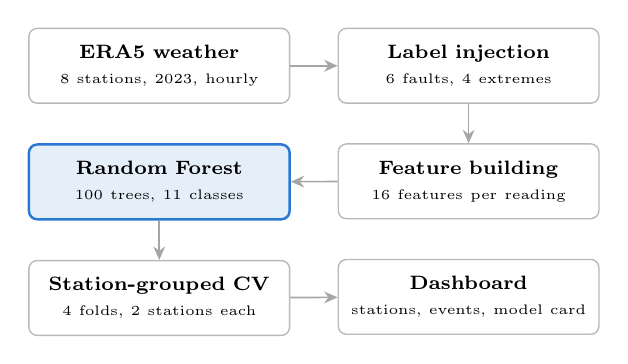
\begin{tikzpicture}[
  font=\scriptsize,
  card/.style={draw=gray!55, fill=white, rounded corners=3pt, align=center,
    text width=3.1cm, minimum height=0.95cm, inner sep=3pt, line width=0.5pt},
  modelcard/.style={card, draw=forest, fill=forest!12, line width=0.9pt},
  flow/.style={-{Stealth[length=1.7mm, width=1.5mm]}, line width=0.6pt, draw=gray!70}
]
\node[card] (a) {\textbf{ERA5 weather}\\[1pt]{\tiny 8 stations, 2023, hourly}};
\node[card, right=0.6cm of a] (b) {\textbf{Label injection}\\[1pt]{\tiny 6 faults, 4 extremes}};
\node[card, below=0.5cm of b] (c) {\textbf{Feature building}\\[1pt]{\tiny 16 features per reading}};
\node[modelcard, below=0.5cm of a] (d) {\textbf{Random Forest}\\[1pt]{\tiny 100 trees, 11 classes}};
\node[card, below=0.5cm of d] (e) {\textbf{Station-grouped CV}\\[1pt]{\tiny 4 folds, 2 stations each}};
\node[card, below=0.5cm of c] (f) {\textbf{Dashboard}\\[1pt]{\tiny stations, events, model card}};
\draw[flow] (a) -- (b);
\draw[flow] (b) -- (c);
\draw[flow] (c) -- (d);
\draw[flow] (d) -- (e);
\draw[flow] (e) -- (f);
\end{tikzpicture}
\caption{Pipeline from raw weather to the dashboard. The classifier is the only learned component.}
\label{fig:pipeline}
\end{figure}

\section{Data}
\subsection{Weather readings}
Hourly temperature, relative humidity, 10\,m wind speed and mean sea-level pressure for 2023 were
taken from the Open-Meteo archive~\cite{openmeteo}, which serves ERA5 reanalysis~\cite{hersbach2020}.
The eight stations (Delhi, Mumbai, Chennai, Hyderabad, Jaipur, Kolkata, Bengaluru, Shimla) cover
arid, coastal, tropical, inland and hill climates. Each station has 8{,}760 hours, giving
280{,}320 sensor readings. Gaps of at most two hours were linearly interpolated before injection, so
the only missing values left are injected dropouts.

\subsection{Injected faults}
Faults affect one sensor at a time, as a real failing instrument does. Each station receives five
episodes of each type at random, non-overlapping times. With $\sigma$ the standard deviation of the
sensor at that station:
\begin{itemize}
\item \emph{bias}: a constant offset of $4$--$7\sigma$ for 24--72\,h;
\item \emph{drift}: an offset growing linearly from $1.5\sigma$ to $5$--$8\sigma$ over 3--7 days;
\item \emph{stuck}: the first value repeated for 12--48\,h;
\item \emph{spike}: about 15\% of hours in a window offset by $6$--$10\sigma$;
\item \emph{precision}: rounding to a step of $0.8$--$1.5\sigma$ plus Gaussian noise;
\item \emph{dropout}: missing readings for 6--24\,h.
\end{itemize}

\subsection{Injected extremes}
Extremes move several sensors together and occur only in their usual season. Each station receives
two of each. The effect follows a half-sine bump over the event, and only hours above 30\% of the
peak are labelled, because the edges are indistinguishable from normal weather. Heat waves
(April--June) raise temperature by about 11\,\textdegree C and lower humidity and pressure; cold
snaps (December--February) lower temperature and raise wind and humidity; storms (June--October)
raise wind and humidity and drop pressure by about 14\,hPa; heavy rain (June--September) saturates
humidity and cools the air.

Table~\ref{tab:data} gives the resulting class balance.

\begin{table}[t]
\caption{Dataset composition}
\label{tab:data}
\centering
\begin{tabular}{@{}lrlr@{}}
\toprule
Class & Readings & Class & Readings \\
\midrule
normal    & 260{,}759 & dropout    & 550 \\
drift     & 4{,}761   & spike      & 432 \\
precision & 2{,}148   & heat wave  & 3{,}918 \\
bias      & 1{,}886   & cold snap  & 2{,}994 \\
stuck     & 1{,}183   & storm      & 933 \\
          &           & heavy rain & 756 \\
\midrule
\multicolumn{4}{@{}l}{normal 93.0\% \quad fault 3.9\% \quad extreme 3.1\%} \\
\bottomrule
\end{tabular}
\end{table}

\section{Methodology}
\subsection{Features}
Every feature is computed per station and sensor from the measured values only. Missing values are
forward-filled for the arithmetic and counted separately. Windows are centred, since the system
analyses a completed record. Table~\ref{tab:features} lists the sixteen features.

\begin{table}[t]
\caption{Features computed for every reading}
\label{tab:features}
\centering
\begin{tabular}{@{}>{\raggedright\arraybackslash}p{2.2cm}>{\raggedright\arraybackslash}p{5.6cm}@{}}
\toprule
Feature & Definition \\
\midrule
value\_z & reading standardised by station and sensor \\
dev\_day & reading minus 24\,h median, in $\sigma$ \\
dev\_week & 24\,h median minus 14-day median, in $\sigma$ \\
jump & change from the previous hour, in $\sigma$ \\
noise\_6h, noise\_day & std of hourly changes over 6\,h and 24\,h \\
flat\_6h & identical consecutive readings in 6\,h \\
missing\_6h & missing readings in 6\,h \\
others\_dev, others\_week & mean $|$dev\_day$|$ and $|$dev\_week$|$ of the other three sensors \\
temp/humid/wind/ press\_week & dev\_week of each sensor at the same station and hour \\
sensor\_code, hour & sensor identity and hour of day \\
\bottomrule
\end{tabular}
\end{table}

The station-level features carry the key physical idea: a fault moves one sensor, while weather
moves several in a recognisable pattern (for example temperature up and humidity down in a heat
wave).

\subsection{Classifier}
A Random Forest~\cite{breiman2001} from scikit-learn~\cite{pedregosa2011} with 100 trees, maximum
depth 20 and at least two samples per leaf predicts one of the eleven classes. Fault and extreme
predictions are grouped for the three-class view. The probability of the normal class gives a
confidence score, $s = 1 - P(\text{normal})$, used to rank flagged readings on the dashboard.

\subsection{Evaluation protocol}
Neighbouring hours are nearly identical, so a random row split would place almost the same reading
in both training and test sets. We instead use 4-fold GroupKFold with the station as the group: each
fold trains on six stations and predicts the remaining two~\cite{roberts2017}. Every reading
therefore receives an out-of-station prediction, and metrics are computed on all 280{,}320 of them.

Because the classes are imbalanced~\cite{he2009}, we report accuracy together with balanced accuracy
(mean per-class recall) and macro F1. Two baselines are used: always predicting \emph{normal}, and an
operational range check that labels a reading as a fault when it is missing or outside fixed limits
(temperature $-5$ to $45$\,\textdegree C, humidity 0--100\%, wind 0--120\,km/h, pressure
950--1050\,hPa).

\section{Results}
\subsection{Overall performance}
Table~\ref{tab:main} compares the classifier with both baselines. On the normal/fault/extreme task
the Random Forest raises balanced accuracy from 44.2\% to 83.4\% and macro F1 from 0.485 to 0.877.
The range check never predicts an extreme and finds few faults, so its accuracy barely exceeds the
majority baseline. On the full eleven-class task the classifier reaches 97.3\% accuracy and a macro
F1 of 0.776.

\begin{table}[t]
\caption{Station-grouped cross-validation results}
\label{tab:main}
\centering
\begin{tabular}{@{}lrrr@{}}
\toprule
Method & Accuracy & Bal.\ acc. & Macro F1 \\
\midrule
Always normal       & 93.0\% & 33.3\% & 0.321 \\
Range check         & 94.3\% & 44.2\% & 0.485 \\
Random Forest (3 groups)  & \textbf{97.9\%} & \textbf{83.4\%} & \textbf{0.877} \\
Random Forest (11 classes) & 97.3\% & 73.8\% & 0.776 \\
\bottomrule
\end{tabular}
\end{table}

Per-station accuracy ranges from 97.5\% (Jaipur) to 98.4\% (Mumbai), and per-station macro F1 from
0.844 to 0.912, so performance carries over to climates the model did not train on.

\subsection{Confusion between groups}
Table~\ref{tab:cm} shows the three-group confusion matrix. False alarms are rare: 0.4\% of normal
readings are flagged. The main error is missed extremes (31.5\% predicted normal), which come mostly
from the shoulders of long events and from short heavy-rain episodes. Faults and extremes are rarely
confused with each other: only 1.5\% of anomalous readings receive the wrong anomaly group.

\begin{table}[t]
\caption{Confusion matrix (rows: truth, share of row)}
\label{tab:cm}
\centering
\begin{tabular}{@{}lrrr@{}}
\toprule
 & Pred.\ normal & Pred.\ fault & Pred.\ extreme \\
\midrule
Normal  & \textbf{99.6\%} & 0.2\% & 0.3\% \\
Fault   & 15.0\% & \textbf{83.0\%} & 1.9\% \\
Extreme & 31.5\% & 1.0\% & \textbf{67.5\%} \\
\bottomrule
\end{tabular}
\end{table}

\subsection{Per-class behaviour}
Fig.~\ref{fig:perclass} shows recall and precision for each class. Faults with a sharp signature are
almost always found: spike (99\%), dropout (98\%) and stuck (87\%). Slow faults are harder: drift
(66\%) and bias (52\%) can resemble a genuine change in the weather. Among extremes, storms (87\%)
are clearest, while heavy rain (19\%) is short and looks like an ordinary humid day.

\begin{figure}[t]
\centering
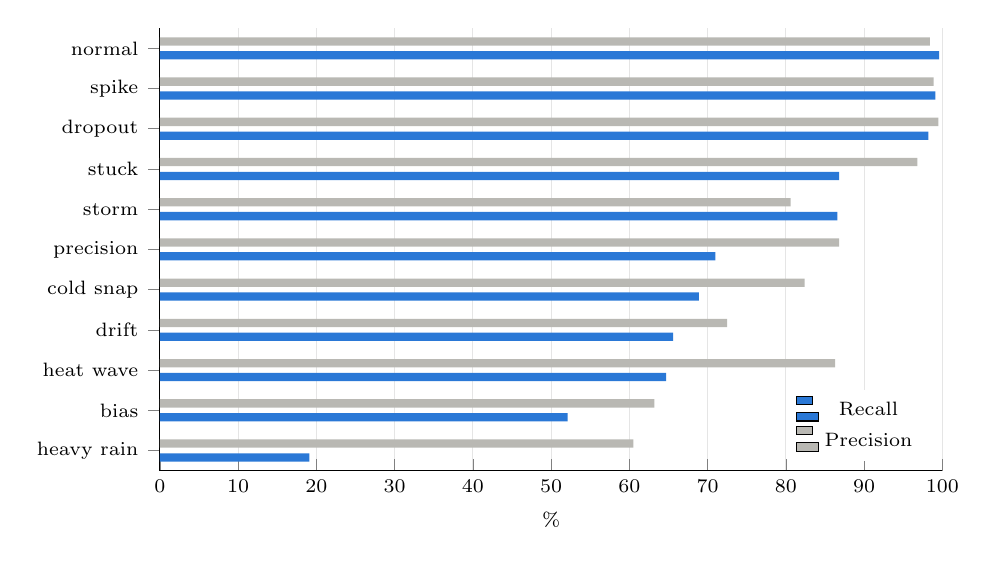
\begin{tikzpicture}
\begin{axis}[
  xbar, width=0.95\columnwidth, height=7.2cm,
  bar width=3pt, xmin=0, xmax=100,
  xlabel={\%}, xlabel style={font=\scriptsize},
  symbolic y coords={heavy rain,bias,heat wave,drift,cold snap,precision,storm,stuck,dropout,spike,normal},
  ytick=data, y tick label style={font=\scriptsize},
  x tick label style={font=\scriptsize},
  legend style={font=\scriptsize, at={(0.98,0.02)}, anchor=south east, draw=none},
  enlarge y limits=0.05, axis x line*=bottom, axis y line*=left,
  xmajorgrids, grid style={gray!20}
]
\addplot[fill=forest, draw=none] coordinates {
  (19.1,heavy rain) (52.1,bias) (64.7,heat wave) (65.6,drift) (68.9,cold snap)
  (71.0,precision) (86.6,storm) (86.8,stuck) (98.2,dropout) (99.1,spike) (99.6,normal)};
\addplot[fill=neutral!60, draw=none] coordinates {
  (60.5,heavy rain) (63.2,bias) (86.3,heat wave) (72.5,drift) (82.4,cold snap)
  (86.8,precision) (80.6,storm) (96.8,stuck) (99.5,dropout) (98.9,spike) (98.4,normal)};
\legend{Recall, Precision}
\end{axis}
\end{tikzpicture}
\caption{Per-class recall and precision under station-grouped cross-validation.}
\label{fig:perclass}
\end{figure}

\subsection{Feature importance}
Fig.~\ref{fig:importance} shows the mean decrease in impurity. The slow deviation \texttt{dev\_week}
is the most useful feature (20.9\%), followed by the station's temperature trend (13.2\%) and the
standardised value (12.3\%). The 24-hour noise feature (9.0\%) drives precision-fault detection, and
the four station-level trend features together contribute 31.0\%, confirming that cross-sensor
context is what separates extremes from faults.

\begin{figure}[t]
\centering
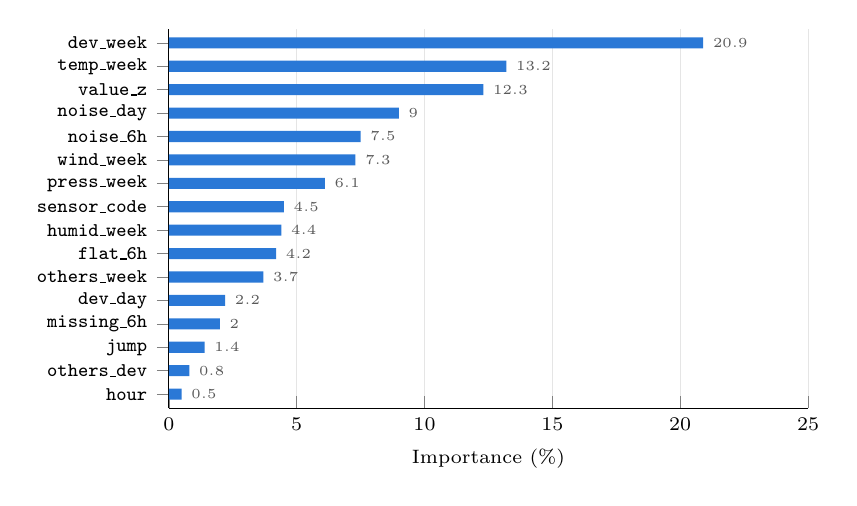
\begin{tikzpicture}
\begin{axis}[
  xbar, width=0.8\columnwidth, height=6.4cm,
  bar width=4pt, xmin=0, xmax=25,
  xlabel={Importance (\%)}, xlabel style={font=\scriptsize},
  ytick={1,...,16},
  yticklabels={hour,others\_dev,jump,missing\_6h,dev\_day,others\_week,flat\_6h,humid\_week,sensor\_code,press\_week,wind\_week,noise\_6h,noise\_day,value\_z,temp\_week,dev\_week},
  y tick label style={font=\scriptsize\ttfamily},
  x tick label style={font=\scriptsize},
  ymin=0.4, ymax=16.6, axis x line*=bottom, axis y line*=left,
  xmajorgrids, grid style={gray!20},
  nodes near coords, nodes near coords style={font=\tiny, text=gray!70!black},
  point meta=x
]
\addplot[fill=forest, draw=none] coordinates {
  (0.5,1) (0.8,2) (1.4,3) (2.0,4) (2.2,5) (3.7,6) (4.2,7) (4.4,8)
  (4.5,9) (6.1,10) (7.3,11) (7.5,12) (9.0,13) (12.3,14) (13.2,15) (20.9,16)};
\end{axis}
\end{tikzpicture}
\caption{Random Forest feature importance (mean decrease in impurity).}
\label{fig:importance}
\end{figure}

\subsection{Episodes}
Consecutive flagged hours on one sensor, with gaps of at most three hours, are merged into episodes
for the dashboard. The model produces 864 episodes (592 fault, 272 extreme), and 80.0\% of them carry
the correct group.

\section{Discussion}
The results support the central idea of the feature design. Sharp, local faults are found from the
sensor's own history, while the decision between \emph{fault} and \emph{extreme} relies on the other
sensors of the same station. The low false-alarm rate (0.4\%) matters operationally, because an
alarm that fires on healthy data is soon ignored.

Accuracy alone is a weak summary here: a model that never flags anything already scores 93.0\%.
Balanced accuracy and macro F1 show the real improvement over the range check, which is close to
the majority baseline because it cannot recognise extremes and misses quiet faults.

\section{Limitations}
The faults and extremes are injected, so their magnitudes and shapes are authored. A model trained on
them learns those patterns, and real failures may be subtler; the reported numbers should be read
as an upper bound for a live network until the model is retrained on logged failures. The weather
itself is reanalysis rather than raw station data, which is smoother than real observations. Centred
windows use a few future hours, which suits offline auditing but would need trailing windows for
real-time alerts. Finally, heavy rain and the early hours of drift remain hard, and longer-context
features are a natural next step.

\section{Conclusion}
A compact supervised pipeline, made of a labelled benchmark built on real ERA5 weather, sixteen
interpretable features and a Random Forest, separates sensor faults from genuine weather extremes
across eight Indian stations. Under station-grouped cross-validation it reaches 97.9\% accuracy,
83.4\% balanced accuracy and a macro F1 of 0.877, well above an operational range check. Future work
will add real station observations, logged instrument failures and trailing-window features for
online monitoring.

\section*{Acknowledgment}
The author thanks the faculty of the School of Computer Science and Engineering, Lovely Professional
University, for guidance during the INT-396 course, and the Open-Meteo and ECMWF teams for open
access to the weather data.

\begin{thebibliography}{00}
\bibitem{ni2009} K. Ni \emph{et al.}, ``Sensor network data fault types,'' \emph{ACM Trans. Sensor
Netw.}, vol. 5, no. 3, pp. 1--29, 2009.
\bibitem{sharma2010} A. B. Sharma, L. Golubchik, and R. Govindan, ``Sensor faults: Detection methods
and prevalence in real-world datasets,'' \emph{ACM Trans. Sensor Netw.}, vol. 6, no. 3, pp. 1--39,
2010.
\bibitem{wmo2004} I. Zahumensk\'{y}, ``Guidelines on quality control procedures for data from
automatic weather stations,'' World Meteorological Organization, Geneva, 2004.
\bibitem{durre2010} I. Durre, M. J. Menne, B. E. Gleason, T. G. Houston, and R. S. Vose,
``Comprehensive automated quality assurance of daily surface observations,'' \emph{J. Appl.
Meteorol. Climatol.}, vol. 49, no. 8, pp. 1615--1633, 2010.
\bibitem{chandola2009} V. Chandola, A. Banerjee, and V. Kumar, ``Anomaly detection: A survey,''
\emph{ACM Comput. Surv.}, vol. 41, no. 3, pp. 1--58, 2009.
\bibitem{liu2008} F. T. Liu, K. M. Ting, and Z.-H. Zhou, ``Isolation forest,'' in \emph{Proc. IEEE
Int. Conf. Data Mining}, 2008, pp. 413--422.
\bibitem{grinsztajn2022} L. Grinsztajn, E. Oyallon, and G. Varoquaux, ``Why do tree-based models
still outperform deep learning on typical tabular data?'' in \emph{Proc. NeurIPS Datasets and
Benchmarks}, 2022.
\bibitem{breiman2001} L. Breiman, ``Random forests,'' \emph{Mach. Learn.}, vol. 45, no. 1,
pp. 5--32, 2001.
\bibitem{openmeteo} P. Zippenfenig, ``Open-Meteo.com Weather API,'' Zenodo, 2023,
doi: 10.5281/zenodo.7970649.
\bibitem{hersbach2020} H. Hersbach \emph{et al.}, ``The ERA5 global reanalysis,'' \emph{Q. J. R.
Meteorol. Soc.}, vol. 146, no. 730, pp. 1999--2049, 2020.
\bibitem{pedregosa2011} F. Pedregosa \emph{et al.}, ``Scikit-learn: Machine learning in Python,''
\emph{J. Mach. Learn. Res.}, vol. 12, pp. 2825--2830, 2011.
\bibitem{roberts2017} D. R. Roberts \emph{et al.}, ``Cross-validation strategies for data with
temporal, spatial, hierarchical, or phylogenetic structure,'' \emph{Ecography}, vol. 40, no. 8,
pp. 913--929, 2017.
\bibitem{he2009} H. He and E. A. Garcia, ``Learning from imbalanced data,'' \emph{IEEE Trans. Knowl.
Data Eng.}, vol. 21, no. 9, pp. 1263--1284, 2009.
\end{thebibliography}

\end{document}
